\documentclass[conference]{IEEEtran}
\IEEEoverridecommandlockouts
\usepackage{cite}
\usepackage{amsmath,amssymb,amsfonts,amsthm}
\usepackage{graphicx}
\usepackage{booktabs}
\usepackage{multirow}
\usepackage{xcolor}
\usepackage[hidelinks]{hyperref}
\newtheorem{proposition}{Proposition}
\newtheorem{corollary}{Corollary}
\graphicspath{{fig/}}

\begin{document}

\title{Is It the Volume or the Smoothing? Closed-Form Analysis and Empirical Evaluation of a Smoothed Accumulation/Distribution Stochastic Oscillator}

\author{
\IEEEauthorblockN{Syahril Fahmi}
\IEEEauthorblockA{Southern Taiwan University of Science and Technology\\
Tainan, Taiwan\\
azairullah701@gmail.com}
\and
\IEEEauthorblockN{\textcolor{red}{[Given name]} Wang}
\IEEEauthorblockA{\textcolor{red}{[Department]}\\
\textcolor{red}{[Institution]}\\
Tainan, Taiwan\\
\textcolor{red}{[email]}}
}

\maketitle

\begin{abstract}
This paper studies the eADL stochastic oscillator, a technical indicator that (i) builds Chaikin's Accumulation/Distribution Line (ADL) with a close-to-close fallback for zero-range bars, (ii) smooths it with an exponential moving average (EMA), (iii) maps it to a bounded $[0,100]$ scale through a stochastic (min--max) transformation, and (iv) produces $K$ and $D$ lines with a two-pass ``re-smoothing'' scheme. We give a formal statement of the indicator and prove that the re-smoothing reduces exactly to first- and second-order linear filters: the re-smoothed $K$ line is a single EMA of the raw stochastic value with gain $\gamma^2$, where $\gamma = 2/(N+1)$, i.e., an equivalent period of $(N+1)^2/2-1$ (49 bars for $N=9$). We verify the closed form against the original JavaScript implementation to machine precision ($<\!10^{-12}$). We then evaluate a long-only $K$/$D$ crossover rule on ten years of daily data for 15 Taiwanese and U.S. assets with realistic Taiwan transaction costs. The eADL oscillator achieves a higher mean Sharpe ratio (0.21) than the classic KD(9,3,3), Stochastic RSI, the Chaikin Oscillator, and its own unsmoothed variants (Wilcoxon $p\le 0.022$), but it underperforms buy-and-hold on all 15 assets and its golden-cross signals show no significant forward-return predictability ($p=0.61$). An ablation shows that applying the same smoothing to price or to On-Balance Volume performs at least as well, indicating that the gain comes from the slow filter rather than from the volume information in the ADL.
\end{abstract}

\begin{IEEEkeywords}
technical analysis, accumulation/distribution line, stochastic oscillator, exponential moving average, digital filters, backtesting, Taiwan stock market
\end{IEEEkeywords}

\section{Introduction}
Volume-based indicators attempt to infer whether a security is being accumulated or distributed by weighting each bar's volume by the location of the close within the bar's range. The best known is Chaikin's Accumulation/Distribution Line (ADL)~\cite{stockcharts_adl,murphy1999}. Because the ADL is a cumulative, unbounded series, it is difficult to read in terms of ``overbought'' or ``oversold'' levels. A common remedy in technical analysis is to apply Lane's stochastic transformation~\cite{lane1984} to a derived series, as in the Stochastic RSI~\cite{chande1994}.

The eADL stochastic oscillator considered here follows that pattern. It was designed by the second author for a charting application and combines four steps: a zero-range fallback for the ADL, EMA smoothing, a stochastic transform, and a two-pass smoothing of the resulting $K$ and $D$ lines that departs from the classic Taiwanese KD weights of $(2/3, 1/3)$.

The individual building blocks are well known. The open question is whether their combination behaves differently from simpler, existing indicators. This paper makes four contributions:
\begin{enumerate}
\item A formal, implementation-faithful definition of the indicator (Section~\ref{sec:def}).
\item A closed-form reduction of the two-pass smoothing to standard linear filters, with its equivalent periods, lags, and stability conditions (Section~\ref{sec:theory}).
\item A cost-aware out-of-the-box evaluation on 15 assets over ten years against five baselines and buy-and-hold (Sections~\ref{sec:setup}--\ref{sec:results}).
\item An ablation that separates the contribution of the volume input from that of the smoothing structure.
\end{enumerate}

\section{Background and Related Work}
\subsection{Accumulation/Distribution Line}
For bar $t$ with high $H_t$, low $L_t$, close $C_t$, and volume $V_t$, the close location value (CLV) is
\begin{equation}
\mathrm{CLV}_t = \frac{(C_t-L_t)-(H_t-C_t)}{H_t-L_t} = \frac{2C_t - H_t - L_t}{H_t-L_t},
\end{equation}
and the ADL accumulates $\mathrm{CLV}_t V_t$~\cite{stockcharts_adl}. The standard definition leaves the case $H_t = L_t$ undefined, and most implementations set $\mathrm{CLV}_t=0$. The Chaikin Oscillator is the difference between the 3- and 10-period EMAs of the ADL~\cite{stockcharts_cho}. On-Balance Volume (OBV)~\cite{granville1963} and Price Volume Trend are related cumulative volume lines.

\subsection{Stochastic Oscillators}
Lane's stochastic~\cite{lane1984} measures where a value lies within its $n$-bar range. The raw value (RSV) is smoothed into a $K$ line and then into a $D$ signal line. In Taiwan the common ``KD'' convention initializes $K=D=50$ and uses the recursion $K_t=\tfrac23K_{t-1}+\tfrac13\mathrm{RSV}_t$, $D_t=\tfrac23D_{t-1}+\tfrac13K_t$. This is an EMA with gain $1/3$, equivalent to a 5-period EMA. Applying the stochastic transform to a derived indicator rather than to price is also established; the Stochastic RSI~\cite{chande1994} is the canonical example.

\subsection{Evidence on Technical Trading Rules}
Brock \emph{et al.}~\cite{brock1992} reported predictive power for simple moving-average rules on historical U.S. data. Later work stressed data-snooping bias~\cite{sullivan1999,white2000} and transaction costs, and Park and Irwin~\cite{park2007} found that profitability largely disappears in more recent and more liquid markets. Multiple testing inflates backtest Sharpe ratios~\cite{bailey2014}. We therefore fix all parameters in advance, report every variant we ran, and test against passive benchmarks.

\section{The eADL Stochastic Oscillator}\label{sec:def}
Let $N$ (\texttt{esp}) be the smoothing period and $n$ (\texttt{KD\_num}) the stochastic window, with defaults $N=n=9$, and let $\gamma = 2/(N+1)$.

\emph{Step 1 (ADL with fallback):} $A_1=0$ and, for $t\ge2$,
\begin{equation}
A_t = A_{t-1} + V_t\cdot
\begin{cases}
\dfrac{2C_t-H_t-L_t}{H_t-L_t}, & H_t\neq L_t,\\[2mm]
\dfrac{C_t}{C_{t-1}}-1, & H_t = L_t.
\end{cases}
\label{eq:adl}
\end{equation}
The fallback is the Price Volume Trend increment. It assigns volume a direction on zero-range bars, which in Taiwan include days locked at the $\pm10\%$ price limit, instead of discarding that volume.

\emph{Step 2 (EMA):} $E_1 = 0$ and $E_t = (1-\gamma)E_{t-1} + \gamma A_t$.

\emph{Step 3 (stochastic transform):} for $t \ge n$, with $M_t=\max_{t-n<j\le t}E_j$ and $m_t=\min_{t-n<j\le t}E_j$,
\begin{equation}
R_t = \begin{cases} 100\,\dfrac{E_t-m_t}{M_t-m_t}, & M_t\neq m_t,\\ 50, & M_t = m_t.\end{cases}
\end{equation}

\emph{Step 4 (two-pass smoothing):} with $K_{n-1}=D_{n-1}=50$ and, for $t\ge n$,
\begin{align}
K'_t &= (1-\gamma)K_{t-1} + \gamma R_t, \label{eq:k1}\\
D'_t &= (1-\gamma)D_{t-1} + \gamma K'_t, \label{eq:d1}\\
K_t  &= (1-\gamma)K_{t-1} + \gamma K'_t, \label{eq:k2}\\
D_t  &= \tfrac{N-3}{N+1}D_{t-1} + \gamma K_t + \gamma D'_t. \label{eq:d2}
\end{align}
Equations~\eqref{eq:k1}--\eqref{eq:d2} follow the order of assignments in the original code. The intermediate values $K'_t$ and $D'_t$ are overwritten in place and never output. Note that $(N-3)/(N+1) = 1-2\gamma$.

\section{Analytical Properties}\label{sec:theory}
\begin{proposition}[Re-smoothed $K$ is a single EMA]\label{prop:k}
For all $t\ge n$,
\begin{equation}
K_t = (1-\gamma^2)K_{t-1} + \gamma^2 R_t .
\end{equation}
\end{proposition}
\begin{proof}
Substitute \eqref{eq:k1} into \eqref{eq:k2}: $K_t = (1-\gamma)K_{t-1} + \gamma(1-\gamma)K_{t-1} + \gamma^2 R_t = (1-\gamma^2)K_{t-1}+\gamma^2R_t$.
\end{proof}

The ``second smoothing'' therefore does not form a cascade of two EMAs, because \eqref{eq:k2} feeds back the final $K_{t-1}$ rather than the previous intermediate value. The result is a single first-order filter with a smaller gain. Matching $\gamma^2 = 2/(N_K+1)$ gives the equivalent EMA period
\begin{equation}
N_K = \frac{(N+1)^2}{2}-1,
\end{equation}
which is 49 bars for the default $N=9$.

\begin{proposition}[$D$ is a second-order linear filter]\label{prop:d}
For all $t\ge n$,
\begin{equation}
D_t = (1-\gamma-\gamma^2)D_{t-1} + \gamma K_t + \gamma^2 K'_t .
\end{equation}
\end{proposition}
\begin{proof}
Substitute \eqref{eq:d1} into \eqref{eq:d2} and use $(N-3)/(N+1)=1-2\gamma$: $D_t=(1-2\gamma)D_{t-1}+\gamma K_t+\gamma(1-\gamma)D_{t-1}+\gamma^2K'_t$, which simplifies to the stated form.
\end{proof}

\begin{corollary}[Boundedness]
The weights in Proposition~\ref{prop:d} sum to one. They are non-negative, so $D_t$ is a convex combination and remains in $[0,100]$, if and only if $\gamma+\gamma^2\le1$. Among integer periods this holds exactly when $N\ge3$. For $N=2$ the coefficient on $D_{t-1}$ is $-1/9$, so the code's weight $(N-3)/(N+1)$ silently imposes $N\ge3$.
\end{corollary}

\emph{Frequency response and lag.} The transfer function of $K$ with respect to $R$ is $H_K(z)=\gamma^2/[1-(1-\gamma^2)z^{-1}]$. Its group delay at DC, equal to the centroid of the impulse response, is $(1-\gamma^2)/\gamma^2 = 24$ bars for $N=9$. Computing the impulse response of $D$ numerically gives a centroid of 26.5 bars. For comparison, the classic Taiwanese KD lags 2 bars ($K$) and 4 bars ($D$). Fig.~\ref{fig:freq} contrasts the magnitude responses. The re-smoothed $K$ attenuates high frequencies far more than either a single EMA with gain $\gamma$ or a true EMA cascade. Table~\ref{tab:equiv} lists equivalent periods for the parameter values used in Section~\ref{sec:results}.

\begin{figure}[t]
\centering
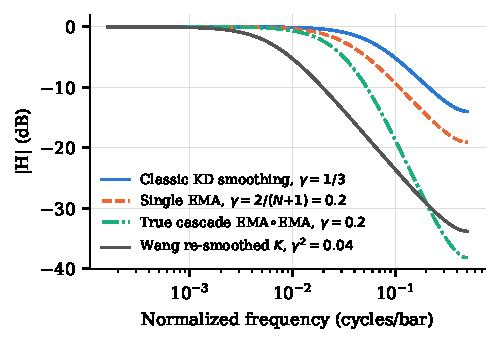
\includegraphics[width=\columnwidth]{freq.pdf}
\caption{Magnitude response of the smoothing filters applied to the raw stochastic value. Wang's re-smoothed $K$ (Proposition~\ref{prop:k}) is a single EMA with gain $\gamma^2$, not a cascade.}
\label{fig:freq}
\end{figure}

\begin{table}[t]
\caption{Equivalent filter parameters of the re-smoothed lines}
\label{tab:equiv}
\centering
\begin{tabular}{rcccc}
\toprule
$N$ & $\gamma$ & $K$ gain $\gamma^2$ & Equiv.\ EMA period $N_K$ & $K$ lag (bars)\\
\midrule
5  & 0.333 & 0.111 & 17.0  & 8.0\\
9  & 0.200 & 0.040 & 49.0  & 24.0\\
14 & 0.133 & 0.018 & 111.5 & 55.3\\
21 & 0.091 & 0.008 & 241.0 & 120.0\\
\bottomrule
\end{tabular}
\end{table}

\section{Experimental Setup}\label{sec:setup}
\subsection{Data}
We downloaded daily OHLCV bars from Yahoo Finance for 3 October 2016 to 2 October 2026, about 2{,}430 bars per asset. The data come through the same endpoint that the charting application uses. The universe has 15 assets: nine Taiwan Stock Exchange instruments (2330 TSMC, 2317 Hon Hai, 2454 MediaTek, 2412 Chunghwa Telecom, 2882 Cathay Financial, 1301 Formosa Plastics, 2303 UMC, 2002 China Steel, and the 0050 ETF), the TAIEX index, four U.S. stocks (AAPL, MSFT, JPM, XOM), and the S\&P~500 index. Bars with missing fields or zero volume were removed. Zero-range bars ($H_t=L_t$) occur on 30 of 36{,}850 bars (0.08\%), all of them on Taiwanese instruments.

\subsection{Implementation and Verification}
The indicator was computed by running the original JavaScript functions \texttt{AccuDistLine\_eADL\_Stochastic} and \texttt{AccuDistLine\_Stochastic} unmodified in Node.js, using 1-based input arrays as the code expects. All other computations used Python. The closed forms of Propositions~\ref{prop:k} and~\ref{prop:d} were implemented independently and compared with the JavaScript output on every asset.

\subsection{Strategies}
Every oscillator is traded with the same long-only rule: hold the asset when $K_t>D_t$ and stay flat otherwise. A signal observed at the close of day $t$ earns the close-to-close return of day $t+1$, so there is no look-ahead. All parameters were fixed at their conventional defaults before testing:
\begin{itemize}
\item \textbf{eADL-KD (Wang)}: the proposed indicator, $N=n=9$.
\item \textbf{ADL-KD (Wang)}: the same code without Step~2, i.e., the stochastic transform applied to the raw ADL.
\item \textbf{eADL-KD single}: Steps 1--3 followed by classic $(2/3,1/3)$ smoothing, which removes the re-smoothing.
\item \textbf{KD(9,3,3)}: the classic Taiwanese KD on price.
\item \textbf{StochRSI}(14,14,3,3)~\cite{chande1994}.
\item \textbf{Chaikin Oscillator}(3,10)~\cite{stockcharts_cho}, long when above zero.
\item \textbf{Buy-and-hold}.
\end{itemize}
Two ablation controls apply \emph{Wang's smoothing} (Propositions~\ref{prop:k}--\ref{prop:d}, $N=9$) to (a) the price RSV of KD(9,3,3) and (b) an EMA-smoothed OBV~\cite{granville1963}.

\subsection{Costs and Metrics}
For Taiwanese instruments we charge the 0.1425\% brokerage fee on both sides and the securities transaction tax on sales: 0.3\% for stocks and 0.1\% for the ETF and the index. U.S. assets are charged 0.05\% per side. We report the compound annual growth rate (CAGR), the annualized Sharpe ratio (zero risk-free rate), maximum drawdown (MDD), trades per year, win rate, and market exposure. The first 60 bars are excluded as warm-up. Differences in Sharpe ratio are tested across the 15 assets with the paired Wilcoxon signed-rank test. Signal predictability is tested with an event study on the 10-day forward return after each golden cross, measured relative to the asset's unconditional mean 10-day return.

\section{Results}\label{sec:results}
\subsection{Verification of the Closed Form}
On all 15 assets the closed-form $K$ and $D$ matched the original JavaScript output to a maximum absolute difference of $1.1\times10^{-13}$, which is floating-point round-off. Propositions~\ref{prop:k} and~\ref{prop:d} therefore describe the deployed implementation exactly. Fig.~\ref{fig:example} shows the result: the eADL-KD lines are visibly smoother and slower than the classic KD.

\begin{figure}[t]
\centering
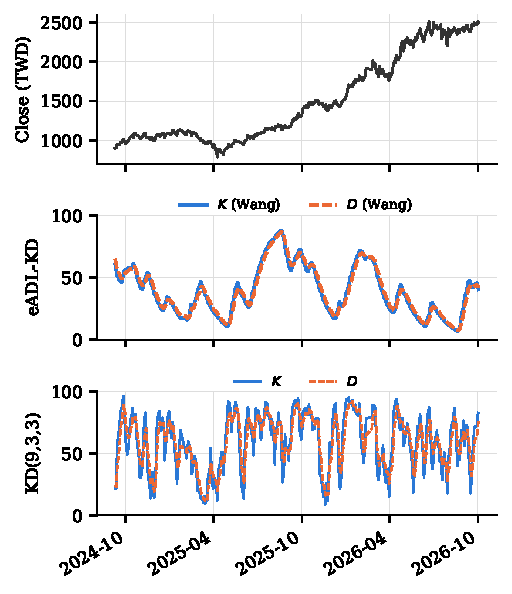
\includegraphics[width=\columnwidth]{example.pdf}
\caption{TSMC (2330.TW), last 500 trading days. Top: close. Middle: eADL-KD ($N=n=9$). Bottom: classic KD(9,3,3).}
\label{fig:example}
\end{figure}

\subsection{Trading Performance}
Table~\ref{tab:main} summarizes the cross-asset means. Among the six non-ablation oscillators, the eADL-KD has the highest Sharpe ratio (0.214), the lowest drawdown (41.5\%), and the fewest trades (7.3 per year). Its Sharpe ratio is significantly higher than those of the classic KD (12 of 15 assets, $p=0.022$), StochRSI (14/15, $p<0.001$), the Chaikin Oscillator (15/15, $p<0.001$), and its own ADL-KD variant without EMA smoothing (14/15, $p<0.001$).

However, \textbf{no oscillator beats buy-and-hold}. Buy-and-hold has a mean Sharpe ratio of 0.687 and a CAGR of 16.7\%, compared with 2.8\% for the eADL-KD, and the eADL-KD has a lower Sharpe ratio than buy-and-hold on every one of the 15 assets (Table~\ref{tab:asset}). Its only advantage over the passive benchmark is a drawdown about 5 percentage points smaller. Fig.~\ref{fig:equity} shows the equity curves for the TAIEX.

\begin{table}[t]
\caption{Cross-asset means (15 assets, Oct.\ 2016--Oct.\ 2026, net of costs)}
\label{tab:main}
\centering
\footnotesize\setlength{\tabcolsep}{2.5pt}
\begin{tabular}{lcccccc}
\toprule
Strategy & CAGR & Sharpe & MDD & Trades/yr & Win & Expo.\\
\midrule
Buy-and-hold          & 16.7\% & 0.687 & 46.2\% & --   & --    & 1.00\\
\midrule
eADL-KD (Wang)        & 2.8\%  & \textbf{0.214} & \textbf{41.5\%} & 7.3  & 44.1\% & 0.52\\
ADL-KD (Wang)         & $-$1.3\% & $-$0.015 & 51.1\% & 12.5 & 40.4\% & 0.51\\
eADL-KD single        & $-$0.9\% & $-$0.026 & 50.8\% & 12.1 & 42.0\% & 0.52\\
KD(9,3,3) price       & $-$0.8\% & $-$0.072 & 52.4\% & 22.6 & 39.4\% & 0.51\\
StochRSI              & $-$4.9\% & $-$0.325 & 61.4\% & 30.4 & 40.8\% & 0.50\\
Chaikin Osc.          & $-$2.3\% & $-$0.101 & 55.4\% & 13.0 & 36.8\% & 0.53\\
\midrule
\multicolumn{7}{l}{\emph{Ablation: Wang smoothing on other inputs}}\\
KD price + Wang sm.   & 4.9\%  & 0.312 & 40.6\% & 12.5 & 39.3\% & 0.52\\
eOBV + Wang sm.       & 5.5\%  & 0.342 & 41.3\% & 7.5  & 42.4\% & 0.53\\
\bottomrule
\end{tabular}
\end{table}

\begin{table}[t]
\caption{Annualized Sharpe ratio by asset (net of costs)}
\label{tab:asset}
\centering
\footnotesize\setlength{\tabcolsep}{3pt}
\begin{tabular}{lcccccc}
\toprule
Asset & B\&H & eADL-KD & eADL & KD & Chaikin & KD+Wang\\
 & & (Wang) & single & (9,3,3) & Osc. & smooth.\\
\midrule
0050.TW & 1.06 & 0.84 & 0.52 & 0.32 & 0.43 & 1.02\\
1301.TW & 0.06 & $-$0.57 & $-$0.96 & $-$0.45 & $-$0.83 & $-$0.35\\
2002.TW & 0.00 & $-$0.53 & $-$1.04 & $-$1.07 & $-$0.86 & $-$0.82\\
2303.TW & 0.94 & 0.35 & 0.41 & 0.25 & 0.23 & 0.79\\
2317.TW & 0.46 & $-$0.02 & $-$0.50 & $-$0.30 & $-$0.30 & 0.20\\
2330.TW & 1.14 & 0.50 & 0.16 & $-$0.08 & 0.10 & 0.65\\
2412.TW & 0.40 & $-$0.27 & $-$0.78 & $-$2.28 & $-$0.97 & $-$0.89\\
2454.TW & 1.02 & 0.69 & 0.43 & 0.59 & 0.31 & 0.45\\
2882.TW & 0.51 & $-$0.27 & $-$0.18 & $-$0.50 & $-$0.53 & 0.10\\
\^{}TWII & 1.04 & 0.48 & 0.33 & 0.36 & 0.11 & 0.79\\
AAPL    & 1.00 & 0.59 & 0.49 & 0.66 & 0.42 & 0.81\\
MSFT    & 0.91 & 0.38 & 0.18 & 0.21 & 0.06 & 0.34\\
JPM     & 0.64 & 0.22 & 0.22 & 0.53 & 0.15 & 0.59\\
XOM     & 0.36 & 0.31 & 0.10 & 0.24 & $-$0.09 & 0.43\\
\^{}GSPC & 0.78 & 0.50 & 0.22 & 0.44 & 0.27 & 0.57\\
\bottomrule
\end{tabular}
\end{table}

\begin{figure}[t]
\centering
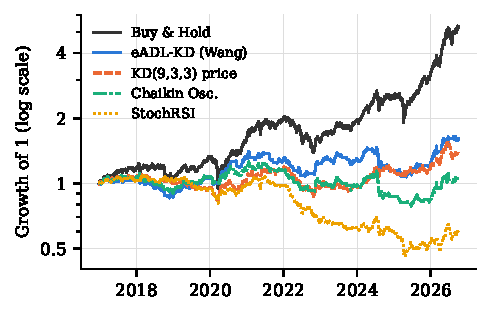
\includegraphics[width=\columnwidth]{equity.pdf}
\caption{Growth of one unit invested in the TAIEX, net of costs.}
\label{fig:equity}
\end{figure}

\subsection{Ablation: Volume or Smoothing?}
The comparisons in Table~\ref{tab:main} isolate each component:
\begin{itemize}
\item \emph{Removing the re-smoothing} (eADL-KD single) lowers the mean Sharpe ratio from 0.214 to $-0.026$ (13/15, $p<0.001$).
\item \emph{Removing the EMA on the ADL} (ADL-KD) lowers it to $-0.015$.
\item \emph{Replacing the ADL by price} while keeping Wang's smoothing \emph{raises} the mean Sharpe ratio to 0.312. The difference from the eADL-KD is not significant ($p=0.17$).
\item \emph{Replacing the ADL by OBV} raises it to 0.342, which is significantly higher than the eADL-KD ($p=0.035$).
\end{itemize}
Taken together, the performance advantage of the eADL-KD comes from the slow smoothing filter of Section~\ref{sec:theory}. The ADL volume information adds nothing measurable beyond that filter.

Fig.~\ref{fig:sharpe} summarizes the ranking.

\begin{figure}[t]
\centering
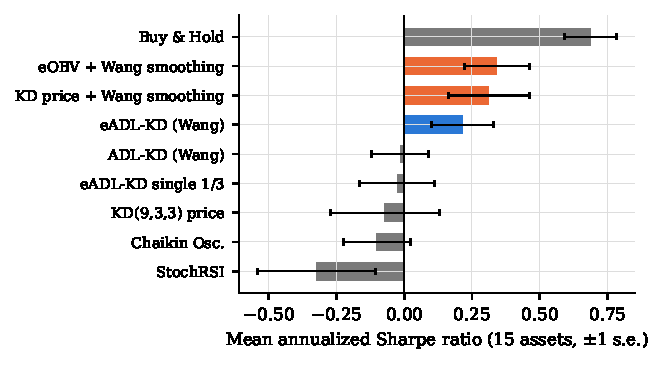
\includegraphics[width=\columnwidth]{sharpe.pdf}
\caption{Mean Sharpe ratio across the 15 assets. Blue: eADL-KD. Orange: Wang's smoothing applied to other inputs.}
\label{fig:sharpe}
\end{figure}

\subsection{Signal Predictability}
The eADL-KD produced 1{,}040 golden crosses. The mean excess 10-day forward return after a cross was $+0.09\%$, with a hit rate of 50.5\% ($t=0.50$, $p=0.61$). None of the other oscillators showed a significant effect either ($p>0.13$). The crossover signals therefore carry no statistically detectable short-horizon information. The backtest gains relative to the faster oscillators come from trading less often and therefore paying fewer costs, not from better timing.

\subsection{Parameter Sensitivity and Subperiods}
Fig.~\ref{fig:sens} shows the mean Sharpe ratio over a grid of $N\in\{5,9,14,21\}$ and $n\in\{9,14,21\}$. Performance rises monotonically with $N$, from 0.06 to 0.41. Larger $N$ means a slower filter, longer holding periods, and behavior closer to buy-and-hold. This is consistent with the cost-reduction explanation, and it means the default $N=9$ is not a tuned optimum. Splitting the sample at 30 September 2021 gives a mean Sharpe ratio of 0.185 in the first half and 0.224 in the second, so the ranking among oscillators is stable over time. Buy-and-hold dominates in both halves (0.709 and 0.675).

\begin{figure}[t]
\centering
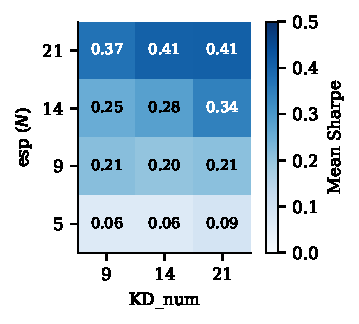
\includegraphics[width=0.75\columnwidth]{sens.pdf}
\caption{Mean Sharpe ratio of eADL-KD across the 15 assets for different smoothing periods $N$ and stochastic windows $n$.}
\label{fig:sens}
\end{figure}

\subsection{Effect of the Zero-Range Fallback}
Replacing the fallback in \eqref{eq:adl} with the conventional $\mathrm{CLV}=0$ changes the $K$ line by at most 1.26 points, on 2454.TW, and by less than 0.3 points on every other affected asset. On daily data from these liquid instruments the fallback is therefore immaterial. It may matter more for illiquid stocks or for intraday bars, where zero-range bars are common.

\section{Discussion}
\emph{Interpretation.} Proposition~\ref{prop:k} recasts the ``second smoothing'' as a reparameterization: for $N=9$ it is a 49-period EMA of the stochastic value. Proposition~\ref{prop:d} shows that the $D$ line is a stable second-order filter whenever $N\ge3$. These facts do not invalidate the indicator. They make it analyzable, and they show that the same behavior can be obtained with one EMA parameter.

\emph{Limitations.} (i) The universe consists of 15 large, liquid survivors, which biases buy-and-hold upward. (ii) We test only one long-only crossover rule, and short selling, overbought/oversold thresholds, and divergence rules are not covered. (iii) Wilcoxon tests across 15 assets have limited power and are not corrected for the eight comparisons. A reality-check bootstrap~\cite{white2000,sullivan1999} would be more rigorous. (iv) Yahoo Finance data may contain errors, and the volume of index series is an aggregate.

\section{Conclusion}
We formalized the eADL stochastic oscillator, proved that its two-pass smoothing reduces to a single EMA of gain $\gamma^2$ for $K$ and a stable second-order filter for $D$, and verified this against the original code to machine precision. In a ten-year, cost-aware test on 15 assets, the indicator outperformed four common oscillators and its own simpler variants. It did not beat buy-and-hold on any asset, and its signals showed no significant predictability. The ablation attributes its advantage to slow smoothing rather than to volume information. Future work should evaluate the indicator on intraday and small-cap data, where zero-range bars and volume effects are larger, and should apply data-snooping-robust inference.

\section*{Acknowledgment}
The authors thank Dr.\ \textcolor{red}{[name]} for comments. \textcolor{red}{[Edit or remove.]}

\begin{thebibliography}{00}
\bibitem{stockcharts_adl} StockCharts.com, ``Accumulation/Distribution Line,'' \emph{ChartSchool}. [Online]. Available: https://chartschool.stockcharts.com/table-of-contents/technical-indicators-and-overlays/technical-indicators/accumulation-distribution-line
\bibitem{murphy1999} J. J. Murphy, \emph{Technical Analysis of the Financial Markets}. New York, NY, USA: New York Institute of Finance, 1999.
\bibitem{stockcharts_cho} StockCharts.com, ``Chaikin Oscillator,'' \emph{ChartSchool}. [Online]. Available: https://chartschool.stockcharts.com/table-of-contents/technical-indicators-and-overlays/technical-indicators/chaikin-oscillator
\bibitem{lane1984} G. C. Lane, ``Lane's stochastics,'' \emph{Technical Analysis of Stocks \& Commodities}, vol.~2, no.~3, 1984.
\bibitem{chande1994} T. S. Chande and S. Kroll, \emph{The New Technical Trader}. New York, NY, USA: Wiley, 1994.
\bibitem{granville1963} J. E. Granville, \emph{Granville's New Key to Stock Market Profits}. Englewood Cliffs, NJ, USA: Prentice-Hall, 1963.
\bibitem{brock1992} W. Brock, J. Lakonishok, and B. LeBaron, ``Simple technical trading rules and the stochastic properties of stock returns,'' \emph{J. Finance}, vol.~47, no.~5, pp.~1731--1764, 1992.
\bibitem{sullivan1999} R. Sullivan, A. Timmermann, and H. White, ``Data-snooping, technical trading rule performance, and the bootstrap,'' \emph{J. Finance}, vol.~54, no.~5, pp.~1647--1691, 1999.
\bibitem{white2000} H. White, ``A reality check for data snooping,'' \emph{Econometrica}, vol.~68, no.~5, pp.~1097--1126, 2000.
\bibitem{park2007} C.-H. Park and S. H. Irwin, ``What do we know about the profitability of technical analysis?'' \emph{J. Economic Surveys}, vol.~21, no.~4, pp.~786--826, 2007.
\bibitem{bailey2014} D. H. Bailey and M. L\'{o}pez de Prado, ``The deflated Sharpe ratio: Correcting for selection bias, backtest overfitting, and non-normality,'' \emph{J. Portfolio Management}, vol.~40, no.~5, pp.~94--107, 2014.
\end{thebibliography}

\end{document}
